\begin{frame}{Check for update safety}%{A Sub-title is optional}
\vspace*{-3mm}%
\begin{center}%
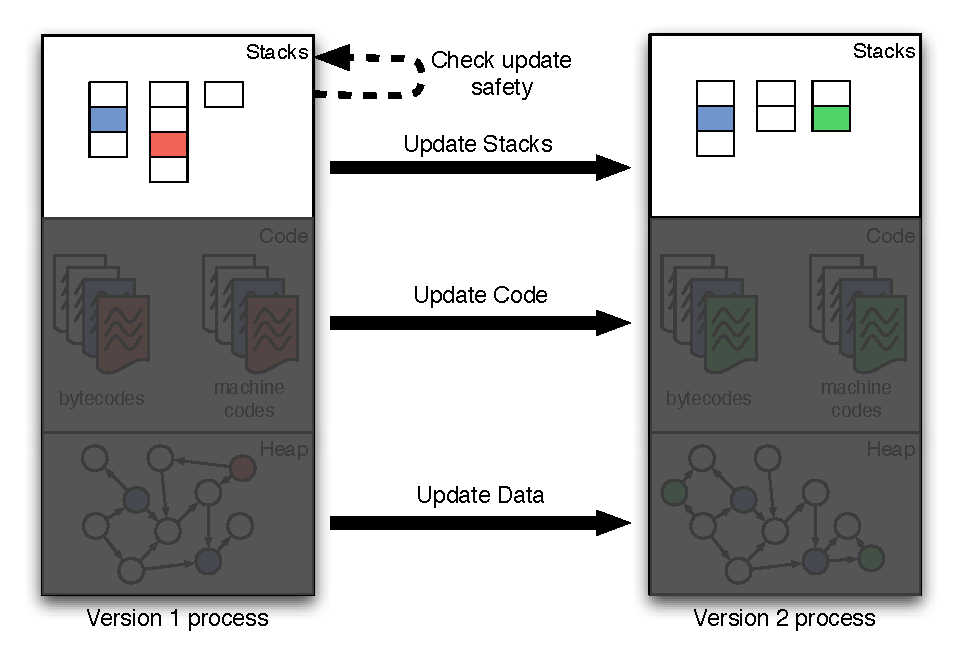
\includegraphics[scale=0.73]{images/process-state/both-process-state-highlight-stack}%
\end{center}%
\end{frame}

\begin{frame}[t,label=suspend]{Safe point for the update}%{A Sub-title is optional}
\begin{textblock*}{0mm}[0,0](90mm,11mm)%
\only<1>{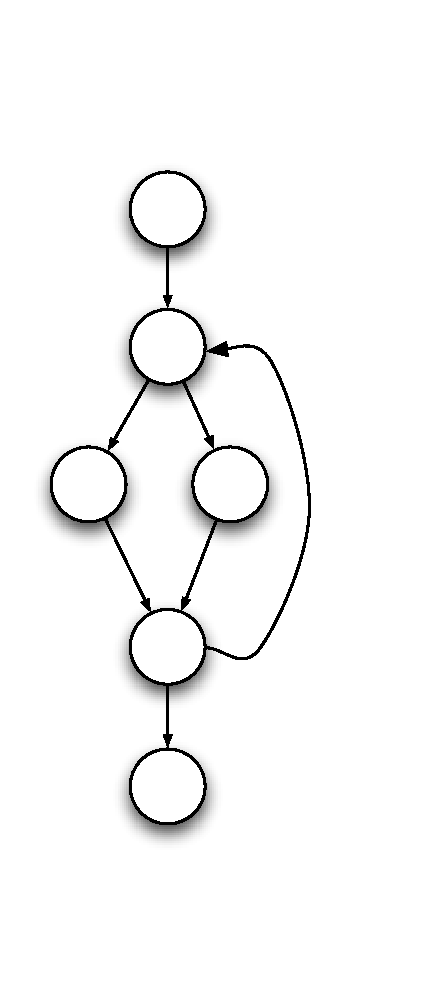
\includegraphics[scale=0.475]{images/yieldpoint/cfg}}%
\only<2->{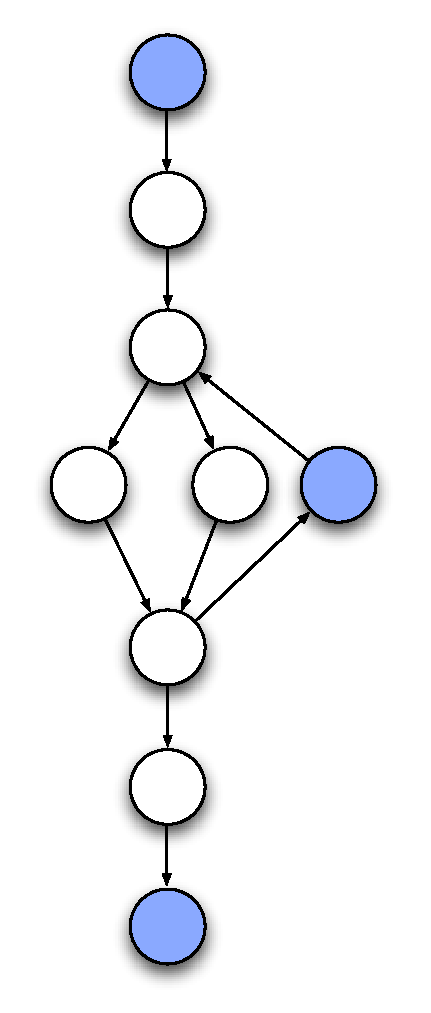
\includegraphics[scale=0.475]{images/yieldpoint/cfg-with-yieldpoint}}%
\end{textblock*}%
\begin{itemize}%
\item Update must be atomic
\item Updates happen at ``safe points''
\item Safe points are VM yield points, \\
      and restrict what methods can be on stack
\item<3> Extend the thread scheduler to \\
      suspend all application threads
\item<3> If any stack has a restricted method, \\
      delay the update
\end{itemize}%
\end{frame}

\begin{frame}[t,fragile]{Restricted methods}%{A Sub-title is optional}
\begin{enumerate}[(1)]
\item Methods changed by the update
\item Methods identified by the user as unsafe based on semantic
information about the application
\begin{block}{}
Install return barriers that trigger DSU upon unsafe method's return
\end{block}
\vspace{2ex}
\item<2> Methods whose bytecode is unchanged, but compiled representation is
      changed by the update
  \begin{itemize}
  \item Offsets of fields and methods hard-coded in machine code
  \item Inlined callees may have changed
  \end{itemize}
\begin{block}{}
Utilize on-stack replacement to recompile base-compiled methods
\end{block}
\end{enumerate}
\end{frame}

% \begin{frame}{Handling restricted methods}%{A Sub-title is optional}
% \vspace*{-2mm}%
% \begin{center}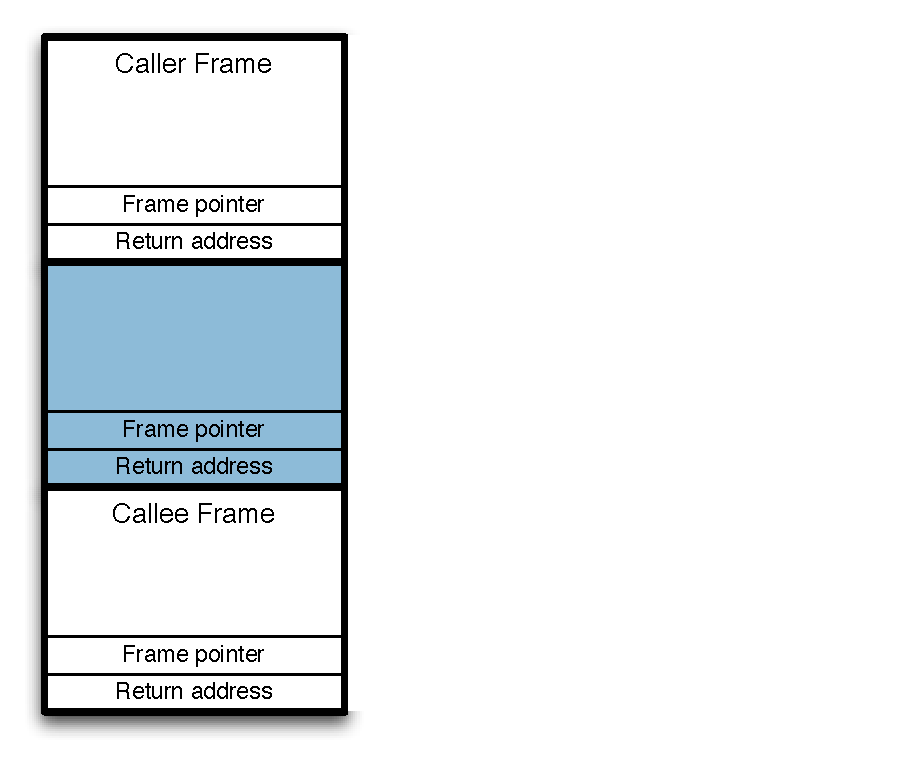
\includegraphics[scale=0.62]{images/stack-smash/stack-frames-overview}\end{center}
% \end{frame}
% 
% \begin{frame}{Installing return barrier for DSU}%{A Sub-title is optional}
% \vspace*{-2mm}%
% \begin{center}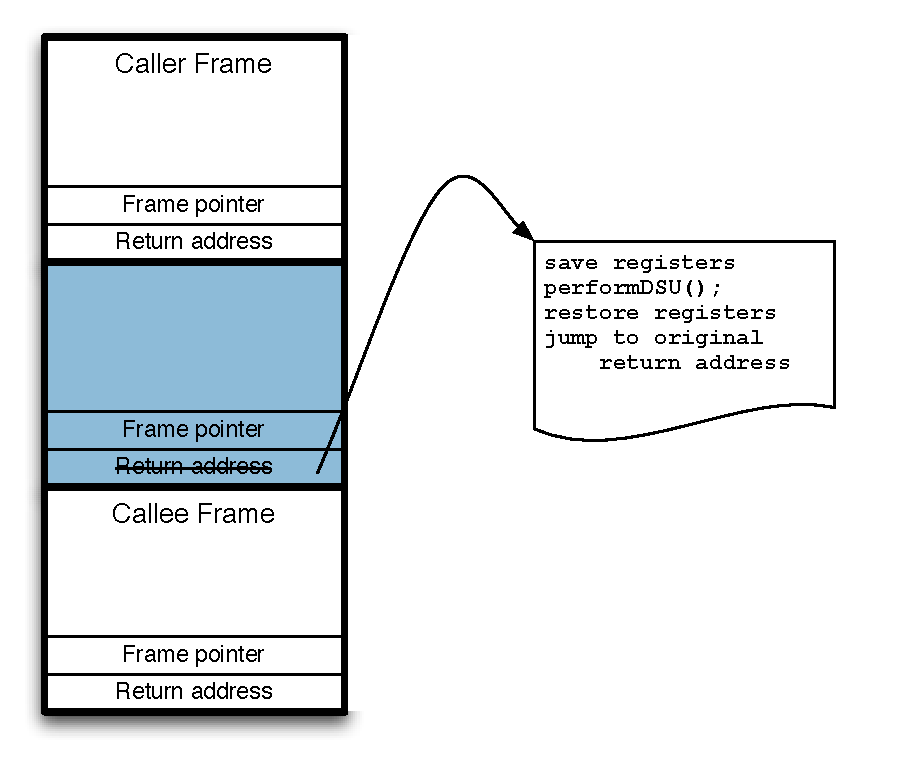
\includegraphics[scale=0.62]{images/stack-smash/return-barrier-overview}\end{center}
% \end{frame}
% 
% \begin{frame}{Performing On-stack replacement}%{A Sub-title is optional}
% \vspace*{-2mm}%
% \begin{center}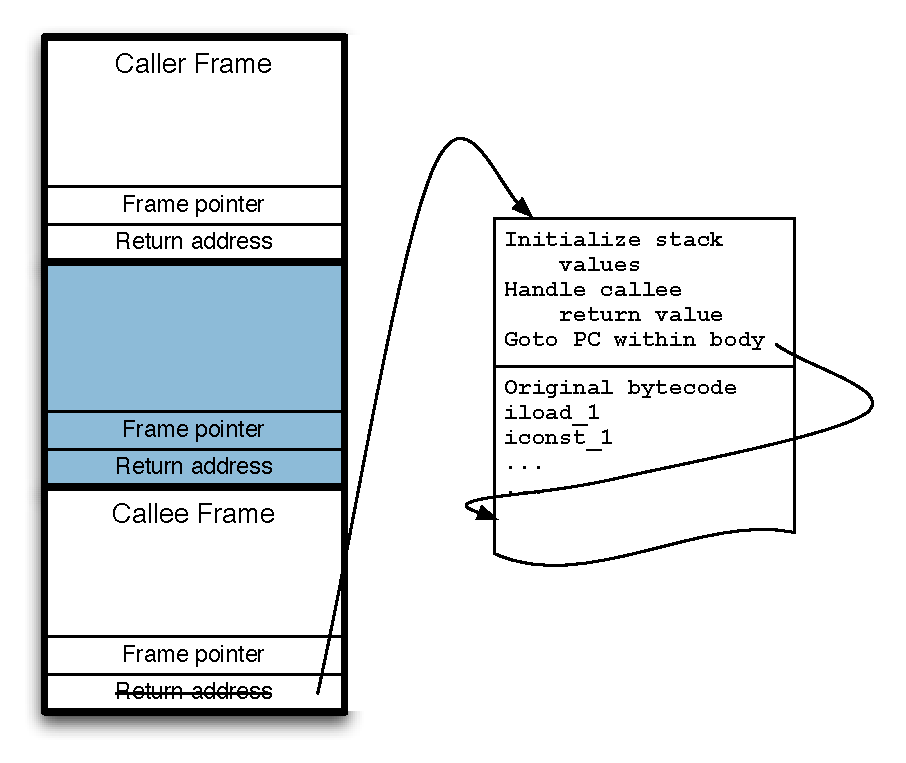
\includegraphics[scale=0.62]{images/stack-smash/osr-overview}\end{center}
% \end{frame}

\begin{frame}{Reaching a safe point}%{A Sub-title is optional}
\hspace*{-3mm}
\begin{center}
\scalebox{0.44}{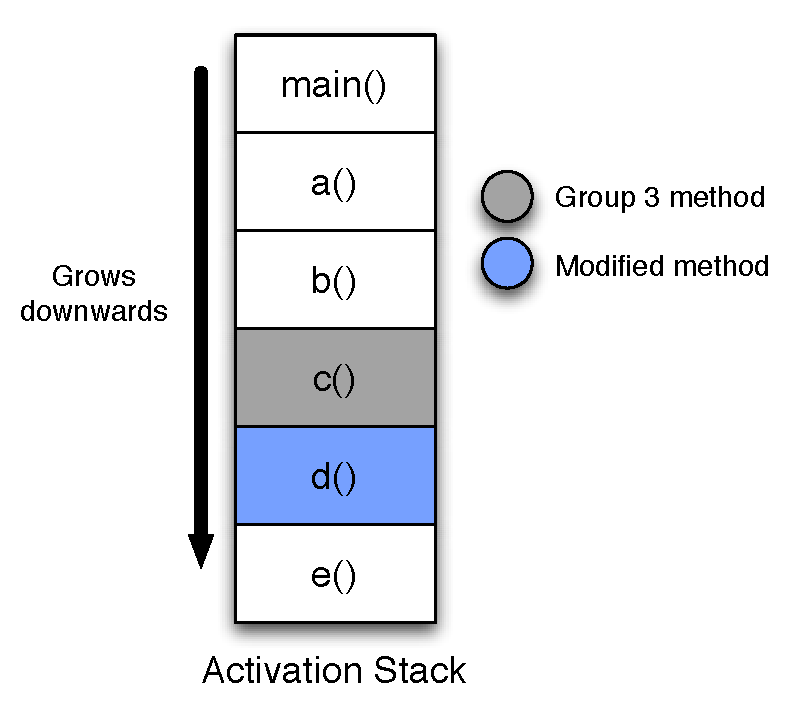
\includegraphics{images/safe-point-call-graph/simple-activation-stack}}
\begin{block}{}
Install a return barrier for d(). Wait till it returns. On-stack replace
new machine code for c().
\end{block}
\end{center}
\end{frame}

% \begin{frame}[c,fragile]{Handling restricted methods}%{A Sub-title is optional}
% \hspace*{-5mm}
% \centering{\scalebox{0.67}{\includegraphics{images/flowchart}}}
% \end{frame}
% 
% \begin{frame}[t,fragile]{On stack replacement in \DSU{}}%{A Sub-title is optional}
% \begin{itemize}
% \item Used in \JikesRVM{} to optimize long running methods
% \item \DSU{} utilizes OSR for DSU
% \item Currently only support baseline-compiled methods
% \item Can OSR any method on stack
% \uncover<2>{
% \item Extract the state of the stack
% \item Construct a new method with a specialized prologue (at the bytecode
% level) that reconstructs the stack
% \item Last instruction of prologue jumps to bytecode where execution should
% resume from
% \item Overwrite the return address to point to the special method
% }
% \end{itemize}
% \end{frame}
% 
% 
% {
% \setbeamercovered{invisible}
% \begin{frame}[t,fragile]{OSR Example}%{A Sub-title is optional}
% \begin{footnotesize}
% \begin{columns}[t]
% 
% \begin{column}{0.4\paperwidth}
% \begin{semiverbatim}
% public class A \{
%   public int foo(int i, B b) \{
%     i = i + 1;
%     i = b.bar(i);
%     i = i + 1;
%     return i;
%   \}
% \}
% \end{semiverbatim}
% 
% \uncover<2-> {
% State: \\
% Thread: \#5 \\
% FP: 0x4ad33e40 \\
% PC: 9 \\
% Locals: i = 5, b = 0x52ae34a0 \\
% Stack vars: S0, S1, ... \\
% }
% \end{column}
% 
% \begin{column}{0.4\paperwidth}
% \begin{semiverbatim}
%  0 iload\_1
%  1 iconst\_1
%  2 iadd
%  3 istore\_1
%  4 aload\_2
%  5 iload\_1
%  6 invokevirtual <B.bar>
%  9 istore\_1
% 10 iload\_1
% 11 iconst\_1
% 12 iadd
% 13 istore\_1
% 14 iload\_1
% 15 ireturn
% \end{semiverbatim}
% \end{column}
% \end{columns}
% \end{footnotesize}
% \end{frame}
% }
% 
% {
% \setbeamercovered{invisible}
% \begin{frame}[t,fragile,shrink=20]{OSR Example}%{A Sub-title is optional}
% \begin{footnotesize}
% \begin{columns}[b]
% 
% \begin{column}{0.4\paperwidth}
% \begin{semiverbatim}
%  0 iload\_1
%  1 iconst\_1
%  2 iadd
%  3 istore\_1
%  4 aload\_2
%  5 iload\_1
%  6 invokevirtual <B.bar>
%  9 istore\_1
% 10 iload\_1
% 11 iconst\_1
% 12 iadd
% 13 istore\_1
% 14 iload\_1
% 15 ireturn
% \end{semiverbatim}
% \end{column}
% 
% \begin{column}{0.4\paperwidth}
% \begin{semiverbatim}
%    ldc 5
%    istore\_0 
%    ldc 0x52ae34a0
%    astore\_1
%    goto 9
%  0 iload\_1
%  1 iconst\_1
%  2 iadd
%  3 istore\_1
%  4 aload\_2
%  5 iload\_1
%  6 invokevirtual <B.bar>
%  9 istore\_1
% 10 iload\_1
% 11 iconst\_1
% 12 iadd
% 13 istore\_1
% 14 iload\_1
% 15 ireturn
% \end{semiverbatim}
% \end{column}
% 
% \end{columns}
% \end{footnotesize}
% \end{frame}
% }
